% Dissertacao de mestrado
% Andressa Sivolella <asivolella@poli.ufrj.br>
% 2016-02-16

\documentclass[msc,numbers]{coppe}
\usepackage{amsmath,amssymb}
\usepackage{hyperref}
\usepackage[latin1]{inputenc}
\usepackage[brazil]{babel}
\usepackage{graphicx}% Include figure files
\usepackage{multirow}
\usepackage{indentfirst}
\usepackage{subfigure}
\usepackage{url}
\usepackage{float}
\usepackage{textcomp}
\usepackage{tikz}
\usepackage{booktabs}
\usepackage{multirow}
\usepackage[table,xcdraw]{xcolor}
\usepackage{pdflscape}
\usetikzlibrary{shapes,arrows}

%\makelosymbols
\makeloabbreviations

\begin{document}
  \title{
    Intelig�ncia Computacional na Avalia��o de C�digos em um Sistema Complexo de Detec��o com Desenvolvimento Colaborativo
  }
  \foreigntitle{
    Computational Intelligence for Source Code Assertion in a Complex System with a Collaborative Development Enviroment
  }
  \author{Andressa Andrea Sivolella}{Gomes}
  \advisor{Prof.}{Jos� Manoel de}{Seixas}{D.Sc.}

  \examiner{Prof.}{Jos� Manoel de Seixas}{D.Sc.}
  \examiner{Prof.}{Alu�zio Fausto Ribeiro Ara�jo}{D.Sc.}
  \examiner{Prof.}{Afonso de Bediaga e Hickman}{D.Sc.}
  \examiner{Prof.}{Luis Henrique Maciel Kosmalski Costa}{D.Sc.}
  \examiner{Pesquisadora}{Carmen L�cia Lodi Maidantchik}{D.Sc.}
  \department{PEE}
  \date{03}{2016}

  \keyword{Minera��o de c�digos}
  \keyword{M�todos ensemble com �rvores}
  \keyword{Plataforma colaborativa}

  \maketitle

  \frontmatter
  %\dedication{A todo mundo, geralz�o.}

  \chapter*{Agradecimentos}

  \begin{abstract}

  Apresenta-se, nesta disserta��o, uma Plataforma web colaborativa, projetada e desenvolvida em um ambiente altamente complexo relacionado a �rea de F�sica de Altas Energias. A referida plataforma tem como um de seus objetivos prover um ambiente para desenvolvimento e compartilhamento de c�digos fonte, que s�o executados em m�quinas separadas do servidor que hospeda a plataforma. Este objetivo foi projetado com a finalidade de n�o sobrecarregar o servidor principal. Mas, c�digos fonte podem conter falhas e a sua n�o identifica��o pr�via, como consequ�ncia, consome recursos computacionais sem necessidade. Neste contexto, esta disserta��o tem como principal objetivo avaliar a possibilidade de aplica��o de algoritmos de aprendizado de m�quina para classificar c�digos fonte que poderiam falhar durante o processo de execu��o. Para atingir tal objetivo, um estudo na �rea de intelig�ncia computacional aplicada a c�digos � realizado, assim como a aplica��o de ferramentas que garantem qualidade no desenvolvimento de software na �rea de F�sica de Altas Energias.

  \end{abstract}

  \begin{foreignabstract}

  In this work it is presented a collaborative web platform, designed and developed in a highly complex environment related to High Energy Physics. That platform has as one of its goals to provide an environment for development and sharing source codes, that are executed on machines separeted from the server hosting this platform. This goal was designed in order to not overload the main server. But source codes may contain flaws and its no prior identification, as a result, consume computer resources unnecessarily. In this context, the main goal of this thesis is to investigate the possibility of applying machine learning algorithms to classify source codes that might fail in an attempt to run, but without running them. To achieve this goal, a study in the area of Computational Intelligence applied to source codes is performed, as well as the application of tools that guarantee quality in software development on High Energy Physics area.

  \end{foreignabstract}

  \tableofcontents
  \listoffigures
  \listoftables
  %\printlosymbols
  \printloabbreviations

  \mainmatter

  \chapter{Introdu��o}
    \section{Motiva��o}
    \section{Objetivos}
    \section{Organiza��o do documento}
  \chapter{A Colabora��o ATLAS do CERN}
    \section{CERN e LHC}
    Fundado em 1954, o CERN (em franc�s \emph{Centre Europ�en pour la Recherch� Nucl�aire}~\cite{CERN}) � o maior centro de pesquisa na �rea de f�sica de part�culas de altas energias no mundo. Atualmente, conta com a participa��o de 38 pa�ses membros e outros pa�ses colaboradores, entre eles o Brasil.

    O LHC (em ingl�s \emph{Large Hadron Collider}~\cite{LHC}) � o maior colisor de part�culas j� constru�do e encontra-se atualmente em opera��o no CERN. Instalado a 175 metros abaixo do solo, consiste em um grande t�nel em formato anelar, com 27 km de per�metro.
    \begin{figure}[htbp]
      \centering
        \includegraphics[width=9.0cm]{images/lhc-upper.png}
        \caption{Representa��o a�rea do LHC e seus detectores no CERN. Extra�do de~\cite{CDS}.}
      \label{LHC}
    \end{figure}
    Quando part�culas s�o eletricamente carregadas e submetidas a pulsos eletromagn�ticos no interior de tubos tem-se o processo de acelera��o de part�culas. Neste processo, as part�culas adquirem acelera��o ao serem envolvidas a campos eletromagn�ticos variantes~\cite{GRIFFITHS}. Em aceleradores circulares, part�culas s�o injetadas e circulam no anel at� atingirem a energia desejada. Diversos experimentos podem ser realizados em determinados pontos de colis�o ao longo da circunfer�ncia. O per�metro do acelerador circular � diretamente proporcional a energia necess�ria na colis�o. Ao atingir a energia desejada, os feixes de part�culas aceleradas em sentidos opostos colidem e, nesse caso, detectores em formato cil�ndrico s�o os mais utilizados. Cada colis�o gera informa��es que devem ser analisadas por especialistas, com objetivos distintos, tais como: identifica��o de sub-part�culas, observa��o de fen�menos e a comprova��o ou a elimina��o de teorias f�sicas. Nos pontos de colis�o, detectores s�o montados para observa��o e coleta de dados. Existem, por exemplo, detectores de calorimetria, para identificar a energia depositada pelas part�culas colisionadas; detectores de tra�os, para observar trajet�rias ap�s colis�es; e detectores de m�ons, respons�veis por absorver tais part�culas.


    A figura~\ref{LHC} ilustra uma representa��o a�rea do LHC. Existem quatro detectores de part�culas instalados em pontos de colis�o ao longo da extens�o do LHC, altamente especializados: ALICE~\cite{ALICE}, ATLAS~\cite{ATLAS}, CMS~\cite{CMS} e LHCb~\cite{SZUMLAK2010}.
    Os detectores ilustrados permitem obter informa��es detalhadas sobre a trajet�ria das part�culas resultantes das colis�es ocorridas e caracter�sticas energ�ticas, sendo poss�vel identificar part�culas. O ATLAS � o maior dos detectores do LHC.

    \section{Experimento ATLAS}
    O ATLAS (em ingl�s \emph{A Toroidal LHC AparatuS})~\cite{ATLAS} � um detector em formato cil�ndrico. O detector pesa aproximadamente 7.000 toneladas, com 44 metros de comprimento por 24 metros de altura. A figura~\ref{ATLAS} ilustra os diversos subsistemas que comp�em o detector ATLAS.

    Cada subsistema apresenta uma caracter�stica espec�fica de acordo com suas funcionalidades. S�o eles, da parte interna para a externa:
    \begin{itemize}
      \item{Detector Interno (ID)}, respons�vel por registrar as trajet�rias
        das part�culas resultantes da colis�o, bem como o momento e o sinal
        da carga, se for o caso;
      \item{Sistema de Calorimetria}, composto pelos calor�metros
        eletromagn�tico (LAr) e hadr�nico de telhas (TileCal). Os calor�metros citados s�o respons�veis por medirem a energia das part�culas resultantes;
      \item{Sistema Magn�tico}, respons�vel por desviar part�culas carregadas
        para medir o momento;
      \item{o Espectr�metro de M�ons}, respons�vel por medir a trajet�ria de
        uma determinada part�cula denominada M�on.
    \end{itemize}

    \begin{figure}[htbp]
      \centering
        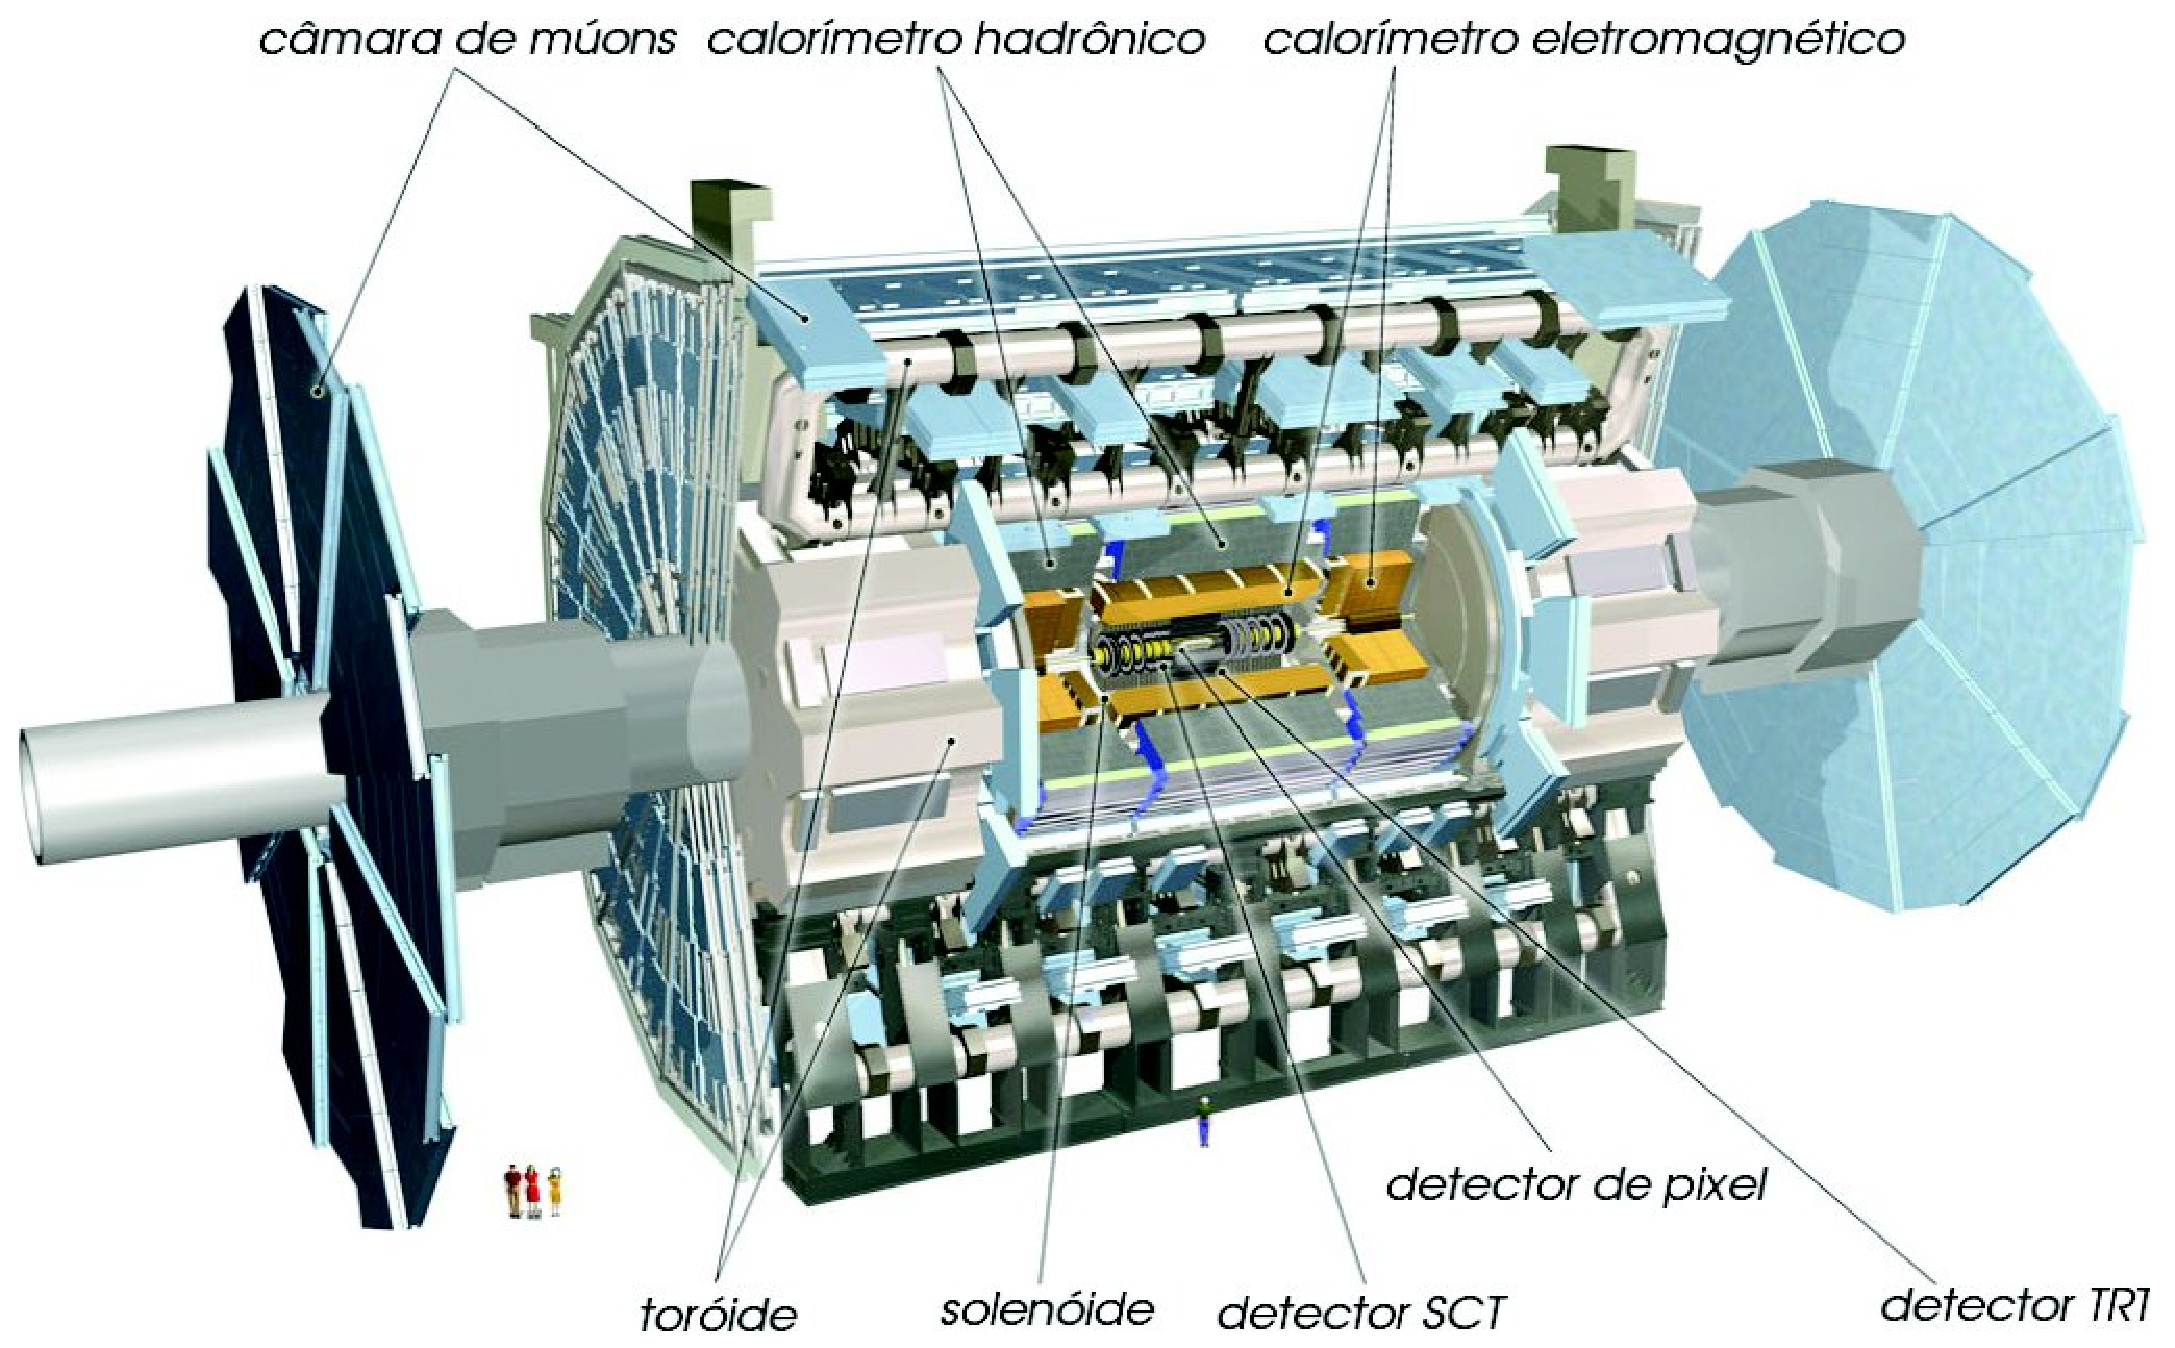
\includegraphics[width=12.0cm,height=8cm]{images/ATLAS_esquema.eps}
        \caption{Esquema do detector ATLAS. Adaptado de~\cite{ATLASPHOTOS}}
      \label{ATLAS}
    \end{figure}
    O sistema de calorimetria do LHC foi projetado para absorver a energia das part�culas que cruzam o detector, sendo o calor�metro hadr�nico de telhas (em ingl�s \emph{Tile Calorimeter} ou TileCal) � o foco deste mestrado.


    \section{Calor�metro Hadr�nico de Telhas (TileCal)}
        \subsection{An�lise \emph{Online} e \emph{Offline}}
        \subsection{A colabora��o TileCal}
  \chapter{Plataforma web Tile-in-ONE}
\label{tio}
Diversos sistemas foram desenvolvidos ao longo das diferentes fases do experimento, cada um com um prop�sito espec�fico~\cite{CHEP2010-DASHBOARD}. A an�lise \emph{online} tem in�cio com a aquisi��o e decis�o acerca do armazenamento dos dados adquiridos, que � responsabilidade do grupo TDAQ (do ingl�s, \emph{Trigger and Data Acquisition})~\cite{jenni2003atlas}. A reconstru��o dos dados pelo software para an�lise \emph{offline} ATHENA~\cite{ATHENA} marca o in�cio da an�lise \emph{offline}. Em seguida, o DQMF (do ingl�s, \emph{Data Quality Monitoring System})~\cite{DQMF} � aplicado e gera automaticamente estados para os PMTs, indicando a qualidade do tubo fotomultiplicador e reduzindo a quantidade de canais que precisam ser analisados. Nesta etapa, gr�ficos s�o gerados para auxiliar o grupo de qualidade de dados do TileCal em sua an�lise \emph{offline}. Um sistema web foi desenvolvido para integrar os resultados gr�ficos gerados durante a etapa de reconstru��o, guiando o grupo de qualidade de dados em suas an�lises. A figura~\ref{dashboard} ilustra sistemas integrados por uma �nica interface web: a figura~\ref{fig:dashboard_1} corresponde a lista de dados reconstru�dos e quais gr�ficos j� est�o dispon�veis para a colabora��o, indicando que a atua��o do ATHENA foi conclu�da; a figura~\ref{fig:dashboard_2} exibe informa��o detalhada sobre um determinado m�dulo, acessado pela interface ilustrada anteriormente. Atrav�s deste sistema web � poss�vel inserir coment�rios relacionados a performance do detector; e a figura~\ref{fig:dashboard_3} ilustra alguns gr�ficos gerados durante a etapa de reconstru��o dos dados.
\begin{figure}[!ht]
  \centering
  \subfigure[Lista dos dados adquiridos.]{
    \includegraphics[width=10cm]{images/screen-capture-5.png}
    \label{fig:dashboard_1}
  }
  \mbox{
    \subfigure[Estados gerados automaticamente pelo DQMF e acesso a informa��es detalhadas.]{
      \includegraphics[width=6.5cm]{images/screen-capture-6.png}
      \label{fig:dashboard_2}
    }
    \subfigure[Gr�ficos gerados para um determinado m�dulo.]{
      \includegraphics[width=6.5cm]{images/screen-capture-7.png}
      \label{fig:dashboard_3}
    }
  }
  \caption{\emph{Dashboard Web System}, desenvolvido em 2010 para integrar as os dados adquiridos e as an�lises do grupo de QD do TileCal. Mais detalhes em~\cite{CHEP2010-DASHBOARD}}
  \label{dashboard}
\end{figure}

Para uma refer�ncia hist�rica, a lista de canais definidos como defeituosos pela colabora��o (\emph{Bad Channels List}) � armazenada no banco de dados de condicionamento, comum a todos os experimentos que comp�em o LHC, o COOL DB~\cite{COOL_DB}. Os sistemas MCWS (do ingl�s, \emph{Monitoring \& Calibration Web System})~\cite{MCWS-CHEP-2012} e DCS (do ingl�s, \emph{Detector Control System})~\cite{DCS-CHEP-2009} apoiam o grupo de qualidade de dados na an�lise dos quase 10.000 PMTs do calor�metro de telhas. O MCWS foi desenvolvido para exibir a lista de canais defeituosos de maneira gr�fica e permite que coment�rios sobre o estado do detector sejam compartilhados. O sistema web DCS foi desenvolvido para monitorar as fontes de alta tens�o que alimentam os PMTs.

� evidente que o cen�rio descrito � composto por diversas ferramentas (web) para apoiar em diferentes aspectos as an�lises e opera��o de forma mais eficiente do TileCal. Tais sistemas foram desenvolvidos em diferentes fases do detector, envolvendo diferentes colaboradores, que n�o necessariamente ainda encontram-se envolvidos em atividades da colabora��o. Al�m disso, a manuten��o de tais ferramentas n�o � garantida pelos mesmos colaboradores contribuintes. Para a colabora��o, seria mais f�cil reunir todas as ferramentas existentes em uma �nica interface, que utilizasse preferencialmente a mesma tecnologia, permitindo inclusive, reutiliza��o de c�digos fonte. Tais requisitos foram contemplados com o projeto e desenvolvimento da Plataforma web Tile-in-ONE.

    \section{Fluxo de dados}

    A Plataforma Tile-in-ONE foi projetada para integrar as diferentes an�lises realizadas pela colabora��o TileCal. Ao fornecer uma estrutura onde os colaboradores podem desenvolver c�digos fonte diretamente atrav�s da web, ela integra diferentes ferramentas em um �nico lugar. Isso garante a escolha da mesma tecnologia para todas as ferramentas desenvolvidas (linguagem Python~\cite{PYTHON}), o que torna a manuten��o da plataforma mais f�cil. Al�m disso, existe o incentivo natural para reutiliza��o de c�digos, uma vez que os desenvolvimentos encontram-se dispon�veis para toda colabora��o. Outra funcionalidade oferecida pela plataforma � o encapsulamento em pacotes de configura��es para acessar bases de dados importantes para as an�lises. Isso permite que colaboradores novos n�o percam tempo aprendendo a acessar a informa��o, mas foquem na an�lise propriamente dita.

    A figura~\ref{fig:dataflow} ilustra o fluxo de dados do Tile-in-ONE. A plataforma oferece a funcionalidade de desenvolvimento de c�digos pela qual os colaboradores podem escrever seus pr�prios programas. Tamb�m � permitida a edi��o de c�digos salvos ou escritos por outros usu�rios. Uma vez que o desenvolvimento do c�digo � conclu�do, o desenvolvedor pode submeter seu c�digo que ser� manipulado no lado do servidor. Este, por sua vez, ir� direcionar o c�digo em quest�o para uma outra m�quina (nesse contexto, m�quinas \emph{slaves}), dependendo dos dados identificados pela plataforma que o c�digo fonte a ser executado deseja acessar. Cada m�quina \emph{slave} est� configurada para acessar um determinado reposit�rio de dados utilizado para as an�lises da colabora��o. Isso permite que os desenvolvedores se abstraiam de configura��es de acesso a tais reposit�rios. A motiva��o para efetuar a execu��o do c�digo fonte em outra m�quina que n�o no servidor � evitar que ocorra sobrecarga no servidor principal e o mais importante: caso o c�digo fonte falhe durante a execu��o, o servidor onde a plataforma est� hospedado n�o fica comprometido. A figura~\ref{fig:dataflow} ilustra ainda, em vermelho, onde esta tese de mestrado ir� atuar. O objetivo � criar uma etapa antes da submiss�o de novos c�digos para m�quinas \emph{slave}, atuando, desta forma, como uma camada de seguran�a cujo intuito � prever quais c�digos v�o falhar sem a necessidade de execut�-los. Esta camada consiste em um novo desenvolvimento e portanto, no momento, qualquer c�digo pode ser submetido para ser executado na m�quina \emph{slave}.

    Uma vez que o servidor web escolhe uma m�quina \emph{slave} esta tenta executar o c�digo fonte submetido e retorna para o servidor web, de maneira estruturada, o que ocorreu durante a execu��o. Neste momento, o desenvolvedor do c�digo fonte pode utilizar objetos gr�ficos tamb�m fornecidos pela plataforma para exibir os resultados recuperados atrav�s de seus c�digos fonte. Enfim, o c�digo fonte, a resposta obtida com a execu��o na m�quina \emph{slave} e os objetos gr�ficos s�o encapsulados em \emph{Plugins} e disponibilizados em \emph{Dashboards} para toda colabora��o.

    \section{Infraestrutura}

    A figura~\ref{fig:infrastructure} ilustra a infraestrutura atual da plataforma web Tile-in-ONE. Destaca-se em vermelho onde este mestrado pretende atuar.

    \begin{figure}[H]
      \centering
      \includegraphics[width=8cm]{images/infrastructure.png}
      \caption{Esquem�tico representando a infraestrutura da plataforma Tile-in-ONE. Em vermelho, a nova camada a ser desenvolvida.}
      \label{fig:infrastructure}
    \end{figure}

    \section{Novo desenvolvimento}

    A plataforma Tile-in-ONE est� atualmente sendo utilizada pelos grupos de calibra��o e qualidade de dados do TileCal. Uma preocupa��o que surgiu ao longo do ano de 2014 foi a execu��o bem sucedida de c�digos fonte sem avalia��o pr�via. Cada c�digo que enfrenta falhas durante sua execu��o na m�quina \emph{slave} acaba consumindo recursos computacionais que podem comprometer o fluxo de dados da plataforma como um todo. A solu��o para tal quest�o levantada � estudada neste mestrado, fazendo uso de t�cnicas de minera��o de c�digos fonte, como abordado no cap�tulo~\ref{code_mining}.

    \begin{figure}[H]
      \centering
      \includegraphics[width=7.5cm, height=24cm]{images/Tile-in-one_dataflow.png}
      \caption{Fluxo de dados da plataforma web Tile-in-ONE.}
      \label{fig:dataflow}
    \end{figure}
  \chapter{Minera��o de c�digos fonte para identifica��o de falhas}
    \section{Sele��o de categorias}
        \subsection{Analisadores Est�ticos}
        \subsection{Medidas estat�sticas e de qualidade}
    \section{Analisadores est�ticos e Minera��o de c�digos no CERN}
  \chapter{Resultados e Conclus�es}
\label{resultados}
    \section{Avalia��o dos Classificadores}
    \label{avaliacao}
  \chapter{Conclus�es}
Independente do desempenho obtido com os 4 classificadores gerados, � poss�vel concluir que o problema de classifica��o de c�digos fonte na plataforma web colaborativa Tile-in-ONE em \emph{execut�vel/n�o execut�vel} pode ser abordado atrav�s de algoritmos de aprendizado de m�quina em \emph{ensemble}. Um pr�ximo passo necess�rio para que tal funcionalidade seja colocada em produ��o seria analisar os c�digos que s�o recorrentemente classificados de maneira equivocada e at� mesmo identificar em qual parte do c�digo exatamente encontra-se o poss�vel \emph{bug}.

Como analisado, existem c�digos fonte, dentre os 512 utilizados para compor o conjunto de dados, que acessam fontes externas de dados (APIs e bancos de dados, por exemplo). Este fato pode ser relevante para o sucesso na execu��o do c�digo e independe das vari�veis de entrada que est�o sendo consideradas neste projeto. Futuramente, pode-se verificar se esse atributo influencia na performance dos classificadores.

A discuss�o de resultados permite concluir que � poss�vel aplicar minera��o de c�digo em um ambiente de F�sica de Altas Energias, extraindo-se apenas caracter�sticas de c�digos fonte.

Atrav�s de um levantamento bibliogr�fico foi poss�vel extrair 11 atributos relacionados a medidas de estat�stica e qualidade de c�digos, dos quais, os mais independentes poss�veis foram selecionados.

Para a classe \emph{n�o execut�vel} o BDT � o m�todo \emph{ensemble} que possui melhor desempenho, quando o F1-score (que � uma pondera��o de precis�o e sensibilidade) � observado. � comum a literatura eleger o BDT como melhor algoritmo dentre os quatro treinados neste projeto.

  \backmatter
  \bibliographystyle{coppe-unsrt}
  \bibliography{dissertacao}
\end{document}